\chapter{Introduction}
\section{Overview}
Foreign exchange is trading of currencies between two countries. For example, when a company in Japan imports some products from the U.S., it exchanges the yen into the U.S. dollar to pay.

In addition to importers and exporters, there are speculators in Forex markets. Individual traders of them often utilize the retail foreign exchange trading (Forex, A.K.A. FX). In Forex, expecting the exchange rate among currencies and taking the long or the short position, a trader tries to get the gain from the difference of the rate between present and future.

The long position is the buying position where he gets the profit if the rate rises (e.g., \$1=Y\llap{=}100 $\Longrightarrow$ \$1=Y\llap{=}120: Profit=Y\llap{=}20). In the opposite case, he suffers a loss. On the other hand, The short position is the selling position where he gets the profit if the rate decrease (e.g., \$1=Y\llap{=}100 $\Longrightarrow$ \$1=Y\llap{=}90 : Profit=Y\llap{=}10). In the opposite case, he suffers a loss. Taking no position is called the square, which means that you get no profit and suffer no loss.

Instead of prediction approach for the future rate, this paper focuses on the strategy to get the profit using Deep Q-learning. The contribution of the thesis is to confirm the performance of moving average as state in the learning because moving average is one of the most basic metrics in the Forex technical analysis.

This thesis has been organized as follows. The rest of this section describes Forex trading system, reinforcement learning, and research motivations. In Section \ref{sec:method_algo}, the algorithm and definitions about Deep Q-learning are detailed. In Section \ref{sec:experiment}, the way of the experiment, dataset, and the evaluation methods are detailed. Section \ref{sec:result} shows the results of the experiment and considers the meanings of them. In Section \ref{sec:conclusion}, conclusions are discussed.

\section{Forex Trading}
\subsection{Details of Forex System}
\label{sec:Forex}
\begin{figure}[htbp]
  \centering
  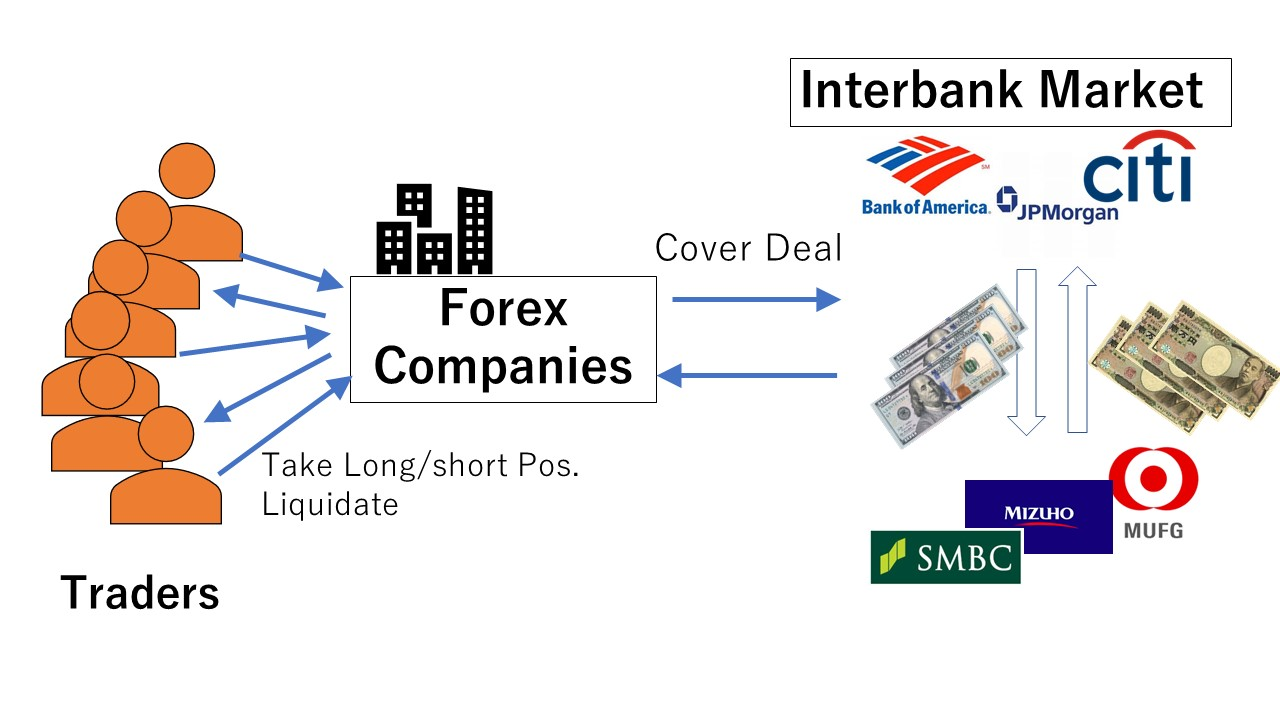
\includegraphics[scale=0.3]{./Figure/ForexEntity.jpg}
  \caption{The overview of Forex entities}
  \label{fig:entities}
\end{figure}
First, we look at the entities of Forex. In Figure \ref{fig:entities} that simplifies the actual situation \cite{bjr2016}, there are traders, Forex companies, and the interbank market. Traders order a Forex company to take a long/short position or to liquidate the position, and then the Forex company conducts the cover deal in the interbank market.

 Ignoring the revenue sources of the forex company such as transaction fee, let us consider the relationship among the long/short position, profit and loss (P/L), and the cover deal.

\begin{figure}
  \centering
  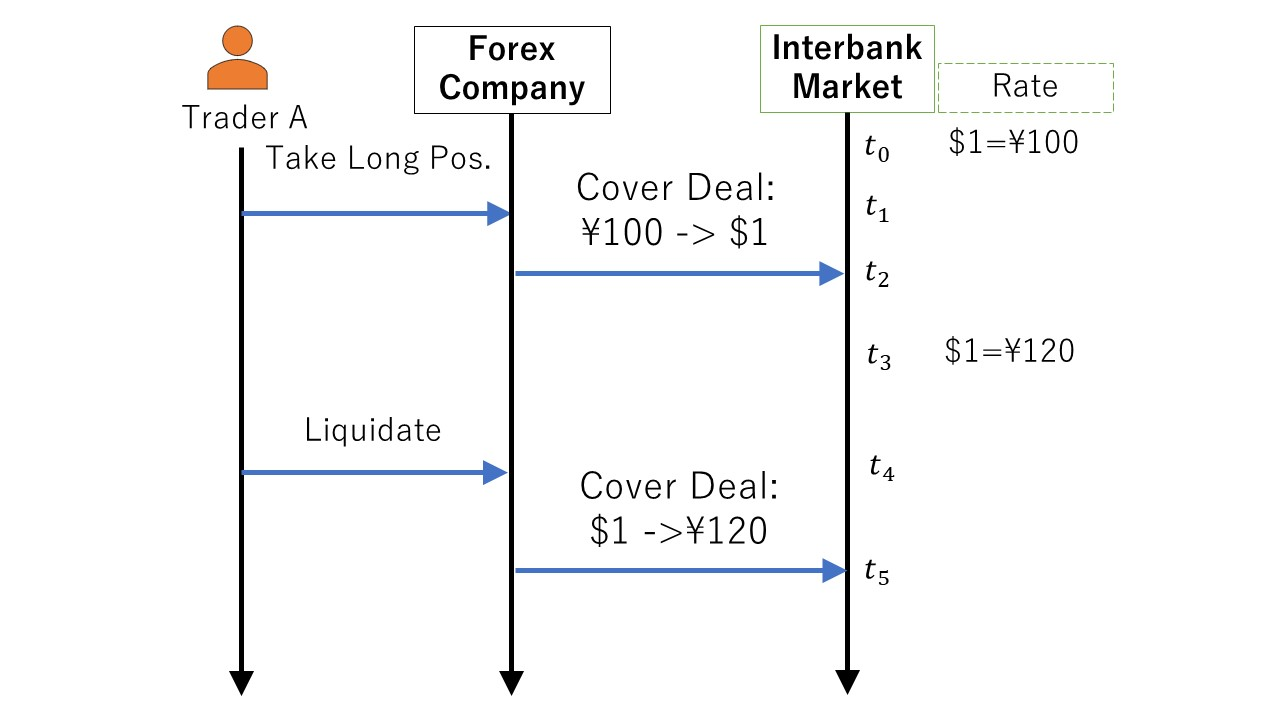
\includegraphics[scale=0.3]{./Figure/Long_CoverDeal1.jpg}
  \caption{Timeline for long position when getting profit}
  \label{fig:lcd1}
\end{figure}

\begin{table}
  \centering
  \caption{P/L and cover deal for long position when getting profit}
  \label{tb:lcd1}
  \begin{tabular}{|c|c|c|c|c|}
  \hline
  \multicolumn{1}{|c|}{} & \multicolumn{3}{c|}{Trader A} & \multicolumn{1}{c|}{} \\
  \cline{2-4}
  Time      & Position & Floating P/L & P/L        & Forex Capital \\
  \hline
  $ t_{0} $ & Square   & Y\llap{=}0   & Y\llap{=}0 & Y\llap{=}100 \\
  $ t_{1} $ & Long     & Y\llap{=}0   & Y\llap{=}0 & Y\llap{=}100 \\
  $ t_{2} $ & Long     & Y\llap{=}0   & Y\llap{=}0 & \$1          \\
  $ t_{3} $ & Long     &+Y\llap{=}20  & Y\llap{=}0 & \$1          \\
  $ t_{4} $ & Square   & Y\llap{=}0   &+Y\llap{=}20& \$1          \\
  $ t_{5} $ & Square   & Y\llap{=}0   &+Y\llap{=}20& Y\llap{=}120 - Y\llap{=}20 = Y\llap{=}100 \\
  \hline
  \end{tabular}
\end{table}

Figure \ref{fig:lcd1} shows that trader A makes a profit of Y\llap{=} 20 on taking the long position. When the trader takes the long position at time $ t_{1} $, the Forex company exchanges yens for dollars as cover deal at time $ t_{2} $. In general, the cover deal means the real trading in the interbank market corresponding to a trader’s position.

And then, suppose that the exchange rate \$1=Y\llap{=}100 changes to \$1=Y\llap{=}120 at time $ t_{3} $. The rate change brings the trader floating P/L. The floating P/L is unrealized profit or loss which floats (changes) in correspondence with the exchange rate and which position he has. For example, if the exchange rate \$1=Y\llap{=}120 at time $ t_{3} $ changes to \$1=Y\llap{=}110 at time $ t_{3.5} $ unlike Figure \ref{fig:lcd1}, his floating P/L as +Y\llap{=}20 also changes to +Y\llap{=}10.

At time $ t_{4} $, the trader liquidates his position to finally realize the profit as +Y\llap{=}20. Liquidating a position means changing the position into the square, finalizing his P/L. And then, the Forex company exchanges dollars for yen as cover deal at time $ t_{5} $ to pay the trader Y\llap{=}20.

There are four patterns for the taking positions and trader's P/L:
\begin{enumerate}
  \item Long position when getting profit $\Longrightarrow$ Figure \ref{fig:lcd1} and Table \ref{tb:lcd1}
  \item Long position when suffering loss $\Longrightarrow$ Figure \ref{fig:lcd2} and Table \ref{tb:lcd2}
  \item Short position when suffering loss $\Longrightarrow$ Figure \ref{fig:scd1} and Table \ref{tb:scd1}
  \item Short position when getting profit $\Longrightarrow$ Figure \ref{fig:scd2} and Table \ref{tb:scd2}
\end{enumerate}

Look at following figures and tables to understand all relationships among positions, P/L, and the cover deal.


\begin{figure}
  \centering
  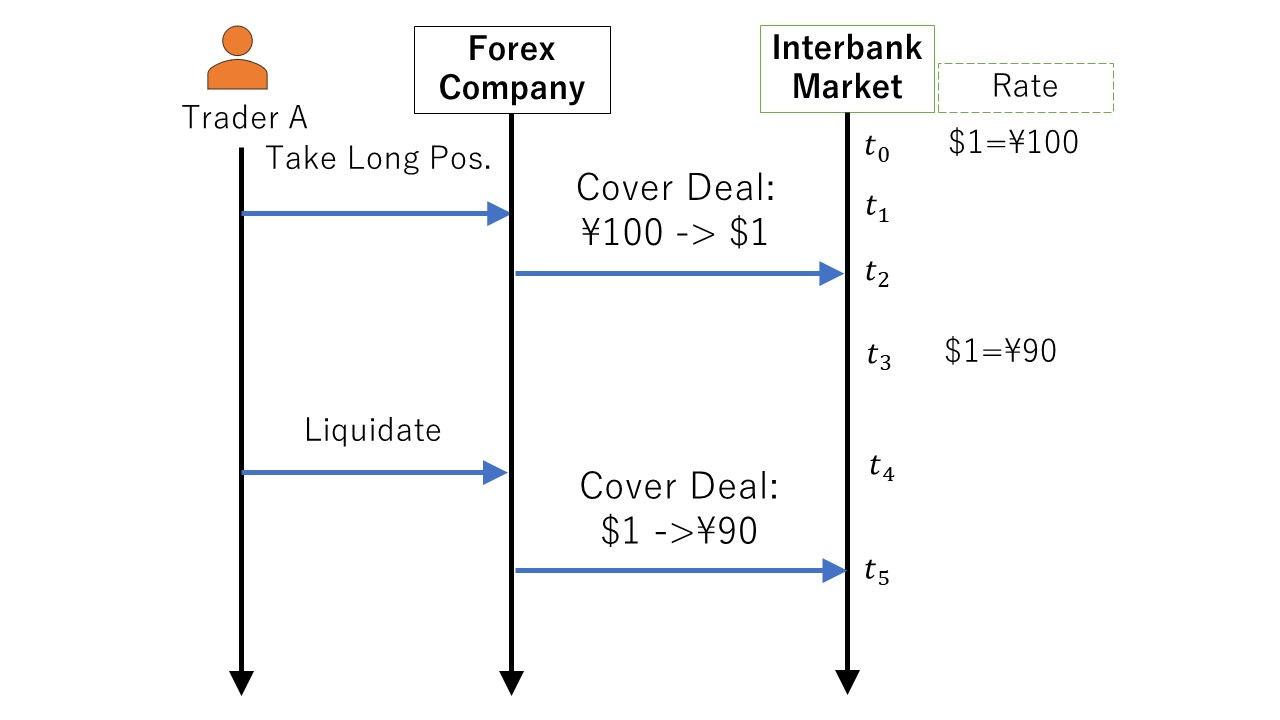
\includegraphics[scale=0.3]{./Figure/Long_CoverDeal2.jpg}
  \caption{Timeline for long position when suffering loss}
  \label{fig:lcd2}
\end{figure}

\begin{table}
  \centering
  \caption{P/L and cover deal for long position when suffering loss}
  \label{tb:lcd2}
  \begin{tabular}{|c|c|c|c|c|}
  \hline
  \multicolumn{1}{|c|}{} & \multicolumn{3}{c|}{Trader A} & \multicolumn{1}{c|}{} \\
  \cline{2-4}
  Time      & Position & Floating P/L & P/L        & Forex Capital   \\
  \hline
  $ t_{0} $ & Square   & Y\llap{=}0   & Y\llap{=}0 & Y\llap{=}100    \\
  $ t_{1} $ & Long     & Y\llap{=}0   & Y\llap{=}0 & Y\llap{=}100    \\
  $ t_{2} $ & Long     & Y\llap{=}0   & Y\llap{=}0 & \$1             \\
  $ t_{3} $ & Long     &-Y\llap{=}10  & Y\llap{=}0 & \$1             \\
  $ t_{4} $ & Square   & Y\llap{=}0   &-Y\llap{=}10& \$1             \\
  $ t_{5} $ & Square   & Y\llap{=}0   &-Y\llap{=}10& Y\llap{=}90 + Y\llap{=}10 = Y\llap{=}100 \\
  \hline
  \end{tabular}
\end{table}


\begin{figure}
  \centering
  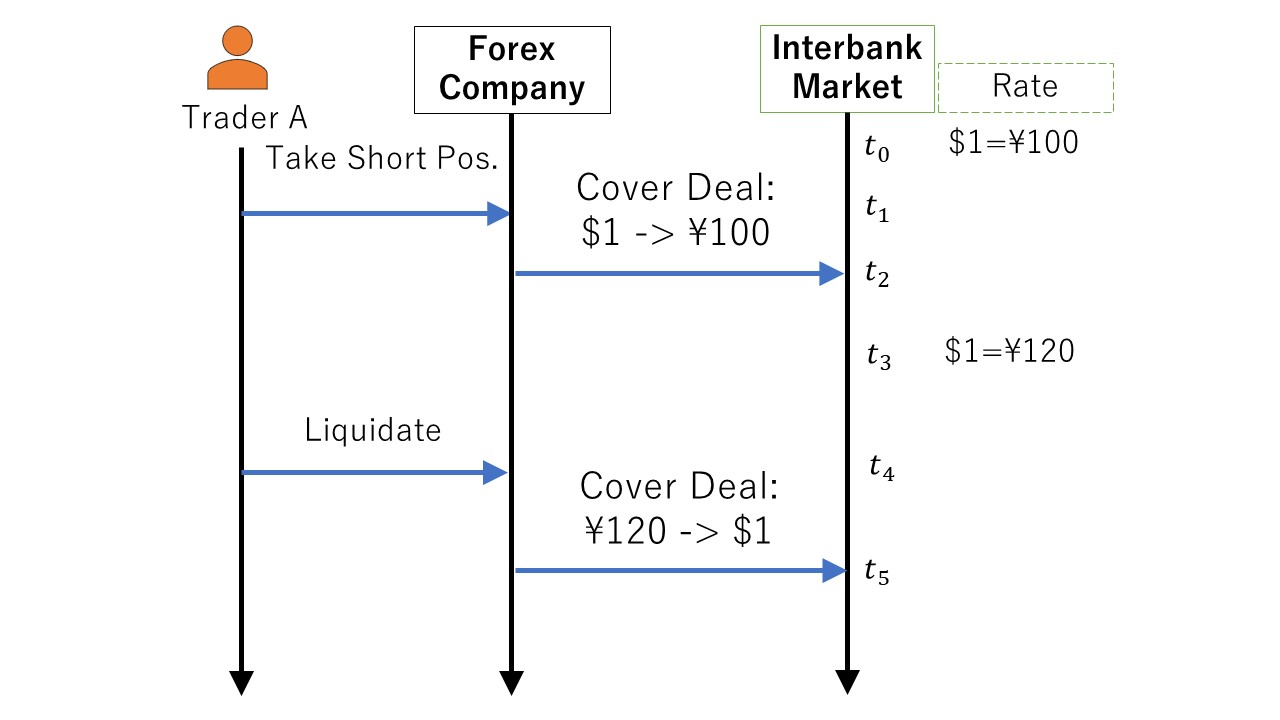
\includegraphics[scale=0.3]{./Figure/Short_CoverDeal1.jpg}
  \caption{Timeline for short position when suffering loss}
  \label{fig:scd1}
\end{figure}

\begin{table}
  \centering
  \caption{P/L and cover deal for short position when suffering loss}
  \label{tb:scd1}
  \begin{tabular}{|c|c|c|c|c|}
  \hline
  \multicolumn{1}{|c|}{} & \multicolumn{3}{c|}{Trader A} & \multicolumn{1}{c|}{} \\
  \cline{2-4}
  Time      & Position & Floating P/L & P/L        & Forex Capital \\
  \hline
  $ t_{0} $ & Square   & Y\llap{=}0   & Y\llap{=}0 & \$1           \\
  $ t_{1} $ & Short    & Y\llap{=}0   & Y\llap{=}0 & \$1           \\
  $ t_{2} $ & Short    & Y\llap{=}0   & Y\llap{=}0 & Y\llap{=}100  \\
  $ t_{3} $ & Short    &-Y\llap{=}20  & Y\llap{=}0 & Y\llap{=}100  \\
  $ t_{4} $ & Square   & Y\llap{=}0   &-Y\llap{=}20& Y\llap{=}100  \\
  $ t_{5} $ & Square   & Y\llap{=}0   &-Y\llap{=}20& Y\llap{=}100 + Y\llap{=}20 = \$1 \\
  \hline
  \end{tabular}
\end{table}


\begin{figure}
  \centering
  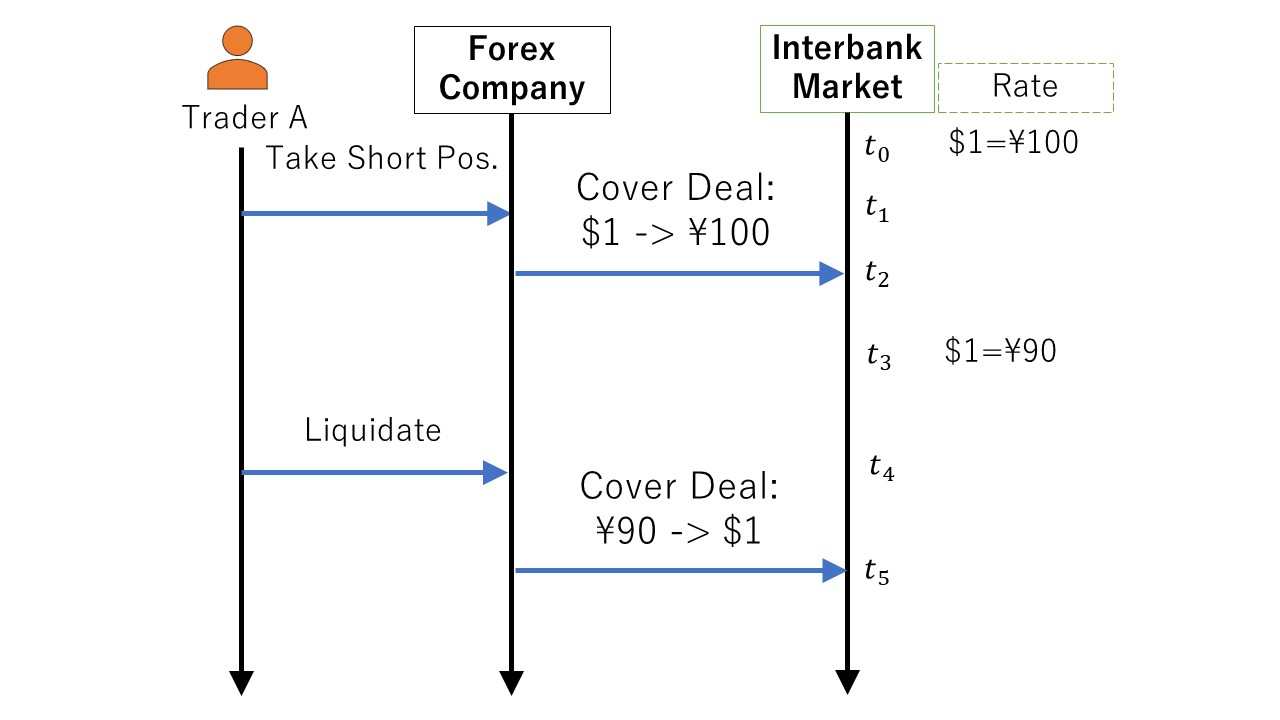
\includegraphics[scale=0.3]{./Figure/Short_CoverDeal2.jpg}
  \caption{Timeline for short position when getting profit}
  \label{fig:scd2}
\end{figure}

\begin{table}
  \centering
  \caption{P/L and cover deal for short position when getting profit}
  \label{tb:scd2}
  \begin{tabular}{|c|c|c|c|c|}
  \hline
  \multicolumn{1}{|c|}{} & \multicolumn{3}{c|}{Trader A} & \multicolumn{1}{c|}{} \\
  \cline{2-4}
  Time      & Position & Floating P/L & P/L        & Forex Capital   \\
  \hline
  $ t_{0} $ & Square   & Y\llap{=}0   & Y\llap{=}0 & \$1           \\
  $ t_{1} $ & Short    & Y\llap{=}0   & Y\llap{=}0 & \$1           \\
  $ t_{2} $ & Short    & Y\llap{=}0   & Y\llap{=}0 & Y\llap{=}100  \\
  $ t_{3} $ & Short    &+Y\llap{=}10  & Y\llap{=}0 & Y\llap{=}100  \\
  $ t_{4} $ & Square   & Y\llap{=}0   &+Y\llap{=}10& Y\llap{=}100  \\
  $ t_{5} $ & Square   & Y\llap{=}0   &+Y\llap{=}10& Y\llap{=}100 - Y\llap{=}10 = \$1 \\
  \hline
  \end{tabular}
\end{table}

The four patterns suggest two features. Firstly, the Forex company keeps the initial capital as Y\llap{=}100 or \$1 without any profit and any loss in any case. It shows that the cover deal literally covers the Forex company from the loss. 

Secondly, the position has the state transition as Figure \ref{fig:pos_trans}.

\begin{figure}[htbp]
  \centering
  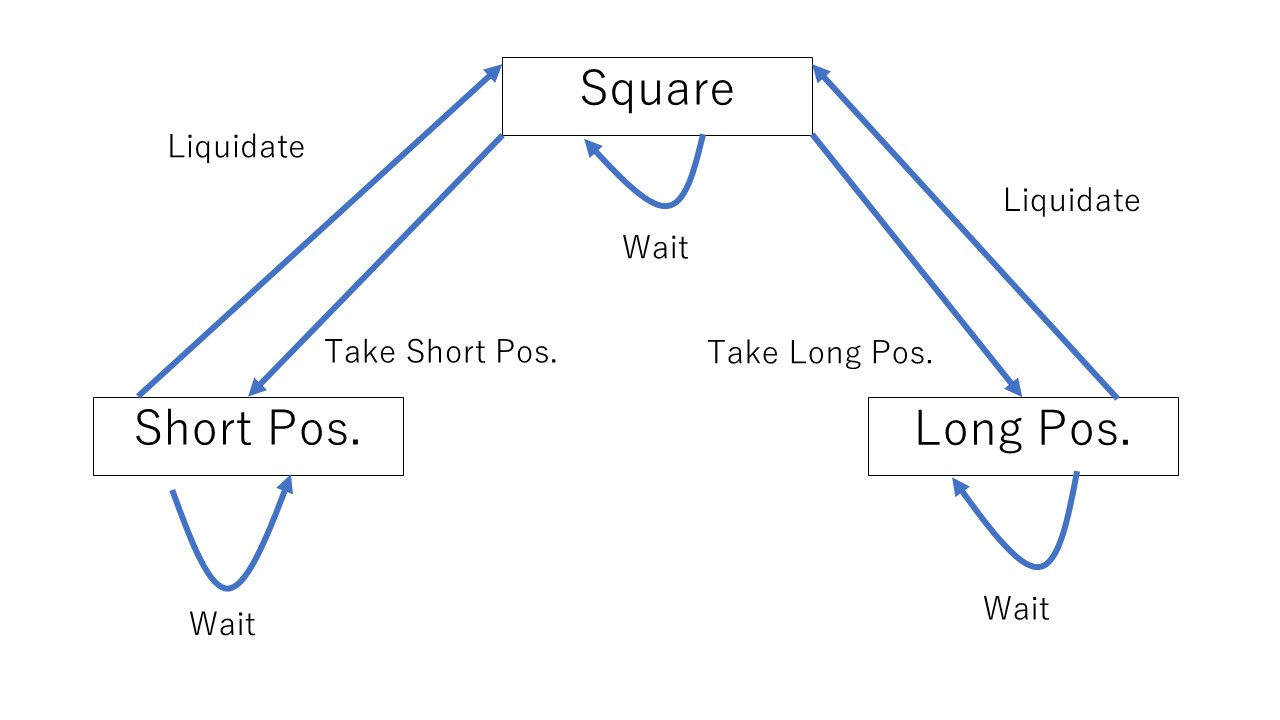
\includegraphics[scale=0.3]{./Figure/pos_transition.jpg}
  \caption{The diagram of the position state transition}
  \label{fig:pos_trans}
\end{figure}


\subsection{Simplification}
Within the scope of this research, all you have to do is to learn the below rules:
\begin{enumerate}
  \item Position State Transition as Figure \ref{fig:pos_trans}
  \item Position and floating P/L
  \begin{itemize}
    \item Long position: The dollar rate rises $\Longrightarrow$ Profit as floating P/L
    \item Long position: The dollar rate decreases $\Longrightarrow$ Loss as floating P/L
    \item Short position: The dollar rate rises $\Longrightarrow$ Loss as floating P/L
    \item Short position: The dollar rate decreases $\Longrightarrow$ Profit as floating P/L
  \end{itemize}
  \item The P/L is finally realized after liquidating the position. 
\end{enumerate}
You do not have to consider the Forex company because it does not affect the trader's P/L.

\section{Reinforcement Learning}
Reinforcement learning (RL) is one of machine learning which learns mapping the pairs of situations-to-actions so as to maximize a reward \cite{sutton2018rl}. In general, the reinforcement learning is modeled as Markov decision process (MDP) like Figure \ref{fig:rl}. At the very beginning, the agent receives the state $ S_{0} $ from the environment, and then the agent takes the action $ A_{0} $. The environment gives the agent the reward $ R_{1} $ and the state $ S_{1} $ in turn, and then the agent takes the action $ A_{1} $, and so on. The (\ref{eq:trajectory}) shows the trajectory: 

\begin{figure}[htbp]
  \centering
  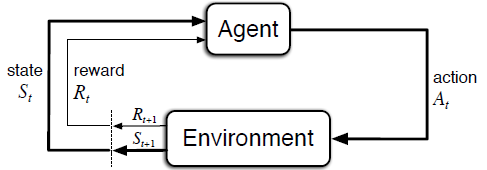
\includegraphics[scale=0.6]{./Figure/rl.png}
  \caption{The agent–environment interaction in a MDP \cite{sutton2018rl}}
  \label{fig:rl}
\end{figure}

\begin{equation}
  \label{eq:trajectory}
  S_{0}, A_{0}, R_{1}, S_{1}, A_{1}, R_{2}, S_{2}, A_{2}, ..., R_{T-1}, S_{T-1}, A_{T-1}, R_{T}, S_{T},
\end{equation}
where $T$ is a final time step \cite{sutton2018rl}. The range of time steps between $0$ and $T$ is called {\it episode} \cite{sutton2018rl}.


\section{Q-learning}
One of the methods in RL is Q-learning. Before explaining it, we introduce some related equations. First, let us define $q_{\pi}$ which is called {\it action-value function for policy} $\pi$ \cite{sutton2018rl} such as

\begin{equation}
  \label{eq:action-value_func}
  q_{\pi}(s,a) := \mathbb{E}[G_{t} | S_{t}=s, A_{t}=s].
\end{equation}

Equation (\ref{eq:action-value_func}) means that $q_{\pi}(s,a)$ outputs the expected return starting from state $s$ and taking the action $a$, after that following policy $\pi$. A policy $\pi$ is a rule where the agent determines the action, and the policy is calculated as conditional probability $\pi(a|s)$.

Second, we introduce {\it optimal action-value function} $q_{*}$, and define it as
\begin{equation}
  \label{eq:opt_av_func}
  q_{*}(s,a) := max \ q_{\pi}(s,a),
\end{equation}
for all $s \in \mathcal{S} $ and $a \in \mathcal{A}(s) $ where $\mathcal{S}$ is set of all nonterminal states and the $\mathcal{A}(s)$ is set of all actions available in state $s$ \cite{sutton2018rl}.

Third, based on Equation \ref{eq:opt_av_func}, it is known to be able to obtain the {\it Bellman optimality equation} for $q_{*}$ \cite{korekara} which is 
\begin{equation}
  \label{eq:Bellman_opt_eq}
  q_{*}(s,a) = \displaystyle \sum_{s'\in \mathcal{S}} p(s'|s,a)[r(s,a,s')+\gamma \ \underset{a' \in \mathcal{A}(s')}{max} \ q_{*}(s',a')].
\end{equation}
The $p(s'|s,a)$ is probability of transition to state $s'$, from state $s$ taking action $a$, the $r(s,a,s')$ is expected immediate reward on transition from $s$ to $s'$ under action $a$, and the $\gamma$ is discount-rate parameter \cite{sutton2018rl}.

Lastly, let us consider Q-learning \cite{korekara} \cite{sutton2018rl} \cite{watkins1989} which is an algorithm defined by
\begin{equation}
  \label{eq:q-learning}
  Q(S_{t},A_{t}) \leftarrow Q(S_{t},A_{t}) + \alpha [R_{t+1} + \gamma \ \underset{a' \in \mathcal{A}(S_{t+1})}{max} \ Q(S_{t+1},a') - Q(S_{t},A_{t})],
\end{equation}
where the $\alpha$ is learning rate.

The (\ref{eq:q-learning}) shows that Q-learning iterates updating the action-value function $Q$ to directly approximate $q_{*}$. When the learning converges, the second term of the (\ref{eq:q-learning}) converges to zero, which means approximating $q_{*}$ since the $R_{t+1} + \gamma \ \underset{a' \in \mathcal{A}(S_{t+1})}{max} \ Q(S_{t+1},a')$ in the (\ref{eq:q-learning}) is similar to Equation (\ref{eq:Bellman_opt_eq}).

The results of updated the action-value function $Q$ are called Q-value and stored into the table which is called Q-table shown as the left side of Figure \ref{fig:QvsDQN}.

\section{Deep Q-learning}
\label{sec:DQL}
It is difficult for Q-learning to solve the problem which has a large state space since the size of Q-table becomes huge \cite{zhang2019end}. This is because all Q-values are allocated as the entire combination of both action and state which are discrete value. Its trouble is called as the curse of dimensionality.

Deep Q Network (DQN) \cite{mnih2013playing}, which is a neural network used by Deep Q-learning, can solve the trouble \cite{zhang2019end}. As the right side of Figure \ref{fig:QvsDQN} shows, Deep Q-learning regards each state element as each DQN input node, which means reducing the size of calculating Q-value. DQN outputs only each Q-value for each action.

\begin{figure}[htbp]
  \centering
  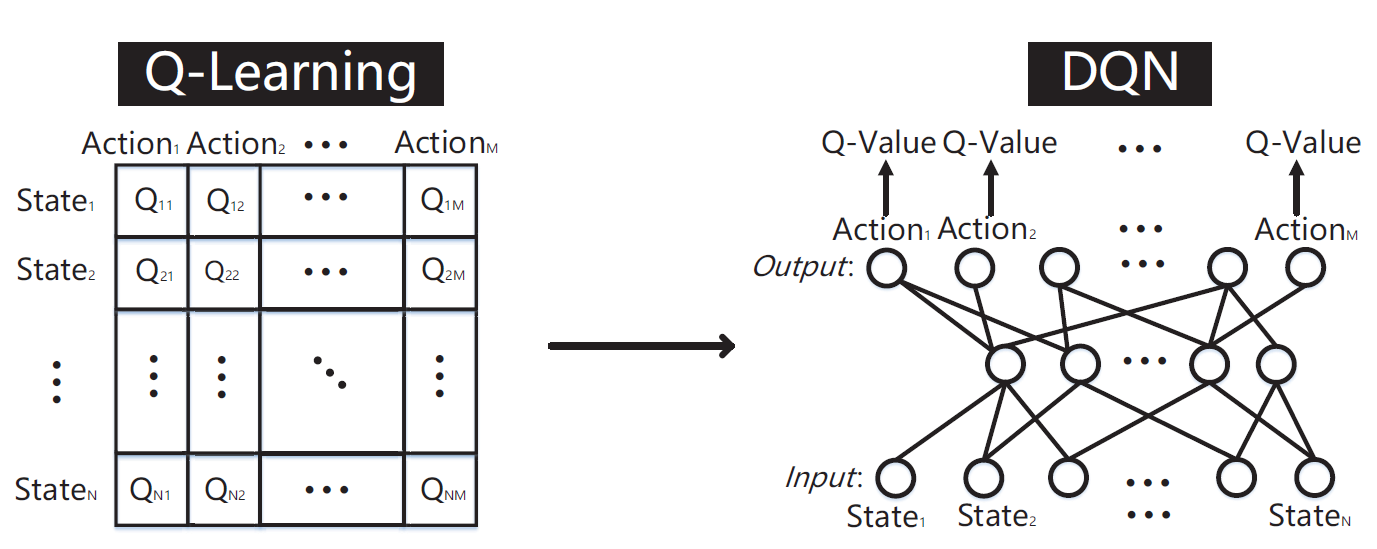
\includegraphics[scale=0.4]{./Figure/QvsDQN.png}
  \caption{Difference between Q-learning and DQN \cite{zhang2019end}}
  \label{fig:QvsDQN}
\end{figure}

\section{Previous Research and Motivation}
\label{sec:motivation}
This paper includes three motivations. First motivation explains the reason to employ RL for Forex trading. 

Before employing RL for finance in earnest, the papers that applied machine learning tended to focus on predicting the future. For example, Arash's survey \cite{bahrammirzaee2010} showed that many papers about trading were related to prediction.

The weakness in the predictive approach is to ignore the option to wait. For example, when a trader cannot be sure the direction of the exchange rate, the best strategy should be to wait without bringing any profit and any loss. However, the predictive approach completely disregards that option.

On the other hand, RL allows the agent to consider waiting as part of actions. This is the reason to employ RL in my research.

Second motivation is utilization of DQN. In terms of RL modeling, Forex trading can be characterized by the continuous of the state while the action is discrete. This is because, in most cases, the state definition includes the exchange rate history which is continuous. On the other hand, the action can be defined as discrete like the position transition in Figure \ref{fig:pos_trans}.

As mentioned in Section \ref{sec:DQL}, DQN is suitable for the modeling where the state and the action are defined as continuous and discrete respectively. This is why this research employs DQN.

The third motivation is to confirm the effect of metrics. Among Forex technical analysis, many metrics are utilized. This research focuses on simple moving average (MA) which is one of the most basic metrics in the analysis \cite{analysisMA}. The experiment verifies whether MA as state element of RL improves the performance of the agent.
